\documentclass{standalone}
\usepackage[margin=1in]{geometry}
\usepackage[hang,small,bf]{caption}
\usepackage{tikz}
\usepackage{braket}
\usetikzlibrary{backgrounds,shadows.blur,fit,decorations.pathreplacing,shapes}

\begin{document}
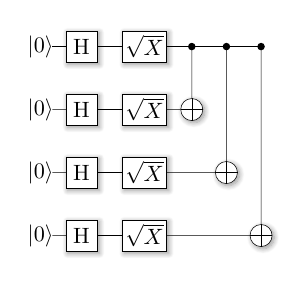
\begin{tikzpicture}[scale=0.8, transform shape]

\tikzstyle{basicshadow}=[blur shadow={shadow blur steps=8, shadow xshift=0.7pt, shadow yshift=-0.7pt, shadow scale=1.02}]\tikzstyle{basic}=[draw,fill=white,basicshadow]
\tikzstyle{operator}=[basic,minimum size=1.5em]
\tikzstyle{phase}=[fill=black,shape=circle,minimum size=0.1cm,inner sep=0pt,outer sep=0pt,draw=black]
\tikzstyle{none}=[inner sep=0pt,outer sep=-.5pt,minimum height=0.5cm+1pt]
\tikzstyle{measure}=[operator,inner sep=0pt,minimum height=0.5cm, minimum width=0.75cm]
\tikzstyle{xstyle}=[circle,basic,minimum height=0.35cm,minimum width=0.35cm,inner sep=-1pt,very thin]
\tikzset{
shadowed/.style={preaction={transform canvas={shift={(0.5pt,-0.5pt)}}, draw=gray, opacity=0.4}},
}
\tikzstyle{swapstyle}=[inner sep=-1pt, outer sep=-1pt, minimum width=0pt]
\tikzstyle{edgestyle}=[very thin]

\node[none] (line0_gate0) at (0.1,-0) {$\Ket{0}$};
\node[none] (line0_gate1) at (0.5,-0) {};
\node[none,minimum height=0.5cm,outer sep=0] (line0_gate2) at (0.75,-0) {};
\node[none] (line0_gate3) at (1.0,-0) {};
\draw[operator,edgestyle,outer sep=0.5cm] ([yshift=0.25cm]line0_gate1) rectangle ([yshift=-0.25cm]line0_gate3) node[pos=.5] {H};
\draw (line0_gate0) edge[edgestyle] (line0_gate1);
\node[none] (line0_gate4) at (1.4000000000000001,-0) {};
\node[none,minimum height=0.5cm,outer sep=0] (line0_gate5) at (1.75,-0) {};
\node[none] (line0_gate6) at (2.1,-0) {};
\draw[operator,edgestyle,outer sep=0.7cm] ([yshift=0.25cm]line0_gate4) rectangle ([yshift=-0.25cm]line0_gate6) node[pos=.5] {$\sqrt{X}$};
\draw (line0_gate3) edge[edgestyle] (line0_gate4);
\node[none] (line1_gate0) at (0.1,-1) {$\Ket{0}$};
\node[none] (line1_gate1) at (0.5,-1) {};
\node[none,minimum height=0.5cm,outer sep=0] (line1_gate2) at (0.75,-1) {};
\node[none] (line1_gate3) at (1.0,-1) {};
\draw[operator,edgestyle,outer sep=0.5cm] ([yshift=0.25cm]line1_gate1) rectangle ([yshift=-0.25cm]line1_gate3) node[pos=.5] {H};
\draw (line1_gate0) edge[edgestyle] (line1_gate1);
\node[none] (line1_gate4) at (1.4000000000000001,-1) {};
\node[none,minimum height=0.5cm,outer sep=0] (line1_gate5) at (1.75,-1) {};
\node[none] (line1_gate6) at (2.1,-1) {};
\draw[operator,edgestyle,outer sep=0.7cm] ([yshift=0.25cm]line1_gate4) rectangle ([yshift=-0.25cm]line1_gate6) node[pos=.5] {$\sqrt{X}$};
\draw (line1_gate3) edge[edgestyle] (line1_gate4);
\node[xstyle] (line1_gate7) at (2.5000000000000004,-1) {};
\draw[edgestyle] (line1_gate7.north)--(line1_gate7.south);
\draw[edgestyle] (line1_gate7.west)--(line1_gate7.east);
\node[phase] (line0_gate7) at (2.5000000000000004,-0) {};
\draw (line0_gate7) edge[edgestyle] (line1_gate7);
\draw (line1_gate6) edge[edgestyle] (line1_gate7);
\draw (line0_gate6) edge[edgestyle] (line0_gate7);
\node[none] (line2_gate0) at (0.1,-2) {$\Ket{0}$};
\node[none] (line2_gate1) at (0.5,-2) {};
\node[none,minimum height=0.5cm,outer sep=0] (line2_gate2) at (0.75,-2) {};
\node[none] (line2_gate3) at (1.0,-2) {};
\draw[operator,edgestyle,outer sep=0.5cm] ([yshift=0.25cm]line2_gate1) rectangle ([yshift=-0.25cm]line2_gate3) node[pos=.5] {H};
\draw (line2_gate0) edge[edgestyle] (line2_gate1);
\node[none] (line2_gate4) at (1.4000000000000001,-2) {};
\node[none,minimum height=0.5cm,outer sep=0] (line2_gate5) at (1.75,-2) {};
\node[none] (line2_gate6) at (2.1,-2) {};
\draw[operator,edgestyle,outer sep=0.7cm] ([yshift=0.25cm]line2_gate4) rectangle ([yshift=-0.25cm]line2_gate6) node[pos=.5] {$\sqrt{X}$};
\draw (line2_gate3) edge[edgestyle] (line2_gate4);
\node[xstyle] (line2_gate7) at (3.0500000000000007,-2) {};
\draw[edgestyle] (line2_gate7.north)--(line2_gate7.south);
\draw[edgestyle] (line2_gate7.west)--(line2_gate7.east);
\node[phase] (line0_gate8) at (3.0500000000000007,-0) {};
\draw (line0_gate8) edge[edgestyle] (line2_gate7);
\draw (line2_gate6) edge[edgestyle] (line2_gate7);
\draw (line0_gate7) edge[edgestyle] (line0_gate8);
\node[none] (line3_gate0) at (0.1,-3) {$\Ket{0}$};
\node[none] (line3_gate1) at (0.5,-3) {};
\node[none,minimum height=0.5cm,outer sep=0] (line3_gate2) at (0.75,-3) {};
\node[none] (line3_gate3) at (1.0,-3) {};
\draw[operator,edgestyle,outer sep=0.5cm] ([yshift=0.25cm]line3_gate1) rectangle ([yshift=-0.25cm]line3_gate3) node[pos=.5] {H};
\draw (line3_gate0) edge[edgestyle] (line3_gate1);
\node[none] (line3_gate4) at (1.4000000000000001,-3) {};
\node[none,minimum height=0.5cm,outer sep=0] (line3_gate5) at (1.75,-3) {};
\node[none] (line3_gate6) at (2.1,-3) {};
\draw[operator,edgestyle,outer sep=0.7cm] ([yshift=0.25cm]line3_gate4) rectangle ([yshift=-0.25cm]line3_gate6) node[pos=.5] {$\sqrt{X}$};
\draw (line3_gate3) edge[edgestyle] (line3_gate4);
\node[xstyle] (line3_gate7) at (3.600000000000001,-3) {};
\draw[edgestyle] (line3_gate7.north)--(line3_gate7.south);
\draw[edgestyle] (line3_gate7.west)--(line3_gate7.east);
\node[phase] (line0_gate9) at (3.600000000000001,-0) {};
\draw (line0_gate9) edge[edgestyle] (line3_gate7);
\draw (line3_gate6) edge[edgestyle] (line3_gate7);
\draw (line0_gate8) edge[edgestyle] (line0_gate9);

\end{tikzpicture}
\end{document}
